%----- Automatically generated by TTool version 2.0 generation date: 05/05/2024 01:56----

\section{Requirements}
\subsection{AVATARRD}
Figures \ref{fig:AVATARRDAVATARRD00} presents ...
\begin{figure*}[htb]
\centering
\includegraphics[width=\textwidth]{img_0_0.png}
\caption{Diagram "AVATARRD"}
\label{fig:AVATARRDAVATARRD00}
\end{figure*}

\section{Analysis}
\subsection{UseCaseDiagram 0}
Figures \ref{fig:UseCaseDiagram 0UseCaseDiagram 010} presents ...
\begin{figure*}[htb]
\centering
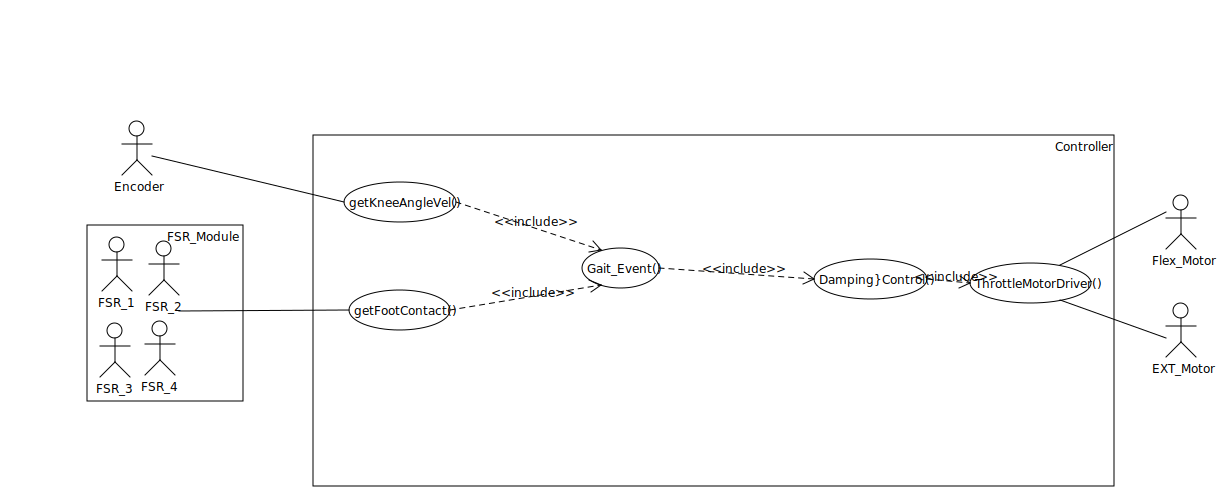
\includegraphics[width=\textwidth]{img_1_0.png}
\caption{Diagram "UseCaseDiagram 0"}
\label{fig:UseCaseDiagram 0UseCaseDiagram 010}
\end{figure*}

\subsection{ActivityDiagram 0}
Figures \ref{fig:ActivityDiagram 0ActivityDiagram 011} presents ...
\begin{figure*}[htb]
\centering
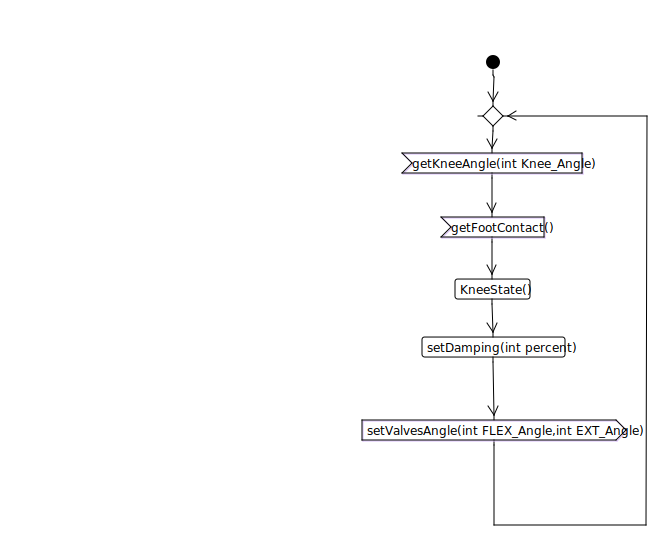
\includegraphics[width=\textwidth]{img_1_1.png}
\caption{Diagram "ActivityDiagram 0"}
\label{fig:ActivityDiagram 0ActivityDiagram 011}
\end{figure*}

\subsection{MyScenario0}
Figures \ref{fig:MyScenario0MyScenario012} presents ...
\begin{figure*}[htb]
\centering
\includegraphics[width=\textwidth]{img_1_2.png}
\caption{Diagram "MyScenario0"}
\label{fig:MyScenario0MyScenario012}
\end{figure*}

\subsection{UseCaseDiagram 1}
Figures \ref{fig:UseCaseDiagram 1UseCaseDiagram 113} presents ...
\begin{figure*}[htb]
\centering
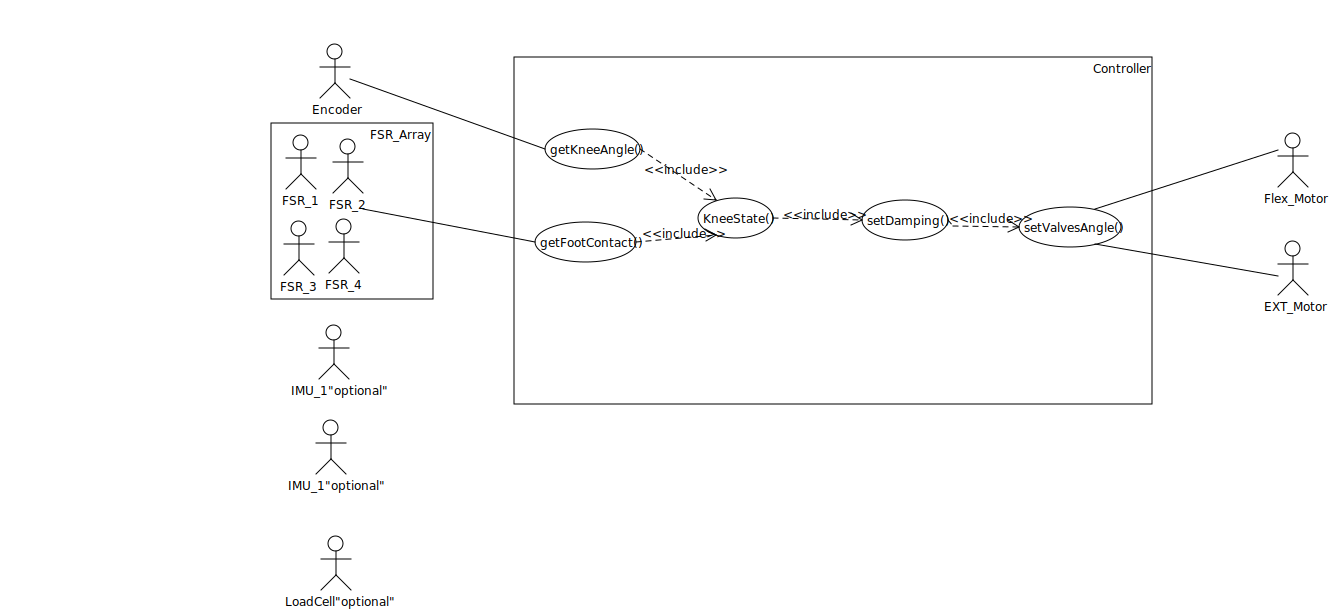
\includegraphics[width=\textwidth]{img_1_3.png}
\caption{Diagram "UseCaseDiagram 1"}
\label{fig:UseCaseDiagram 1UseCaseDiagram 113}
\end{figure*}

\section{Design}
\subsection{Block Diagram}
Figures \ref{fig:Block DiagramBlock Diagram20} presents ...
\begin{figure*}[htb]
\centering
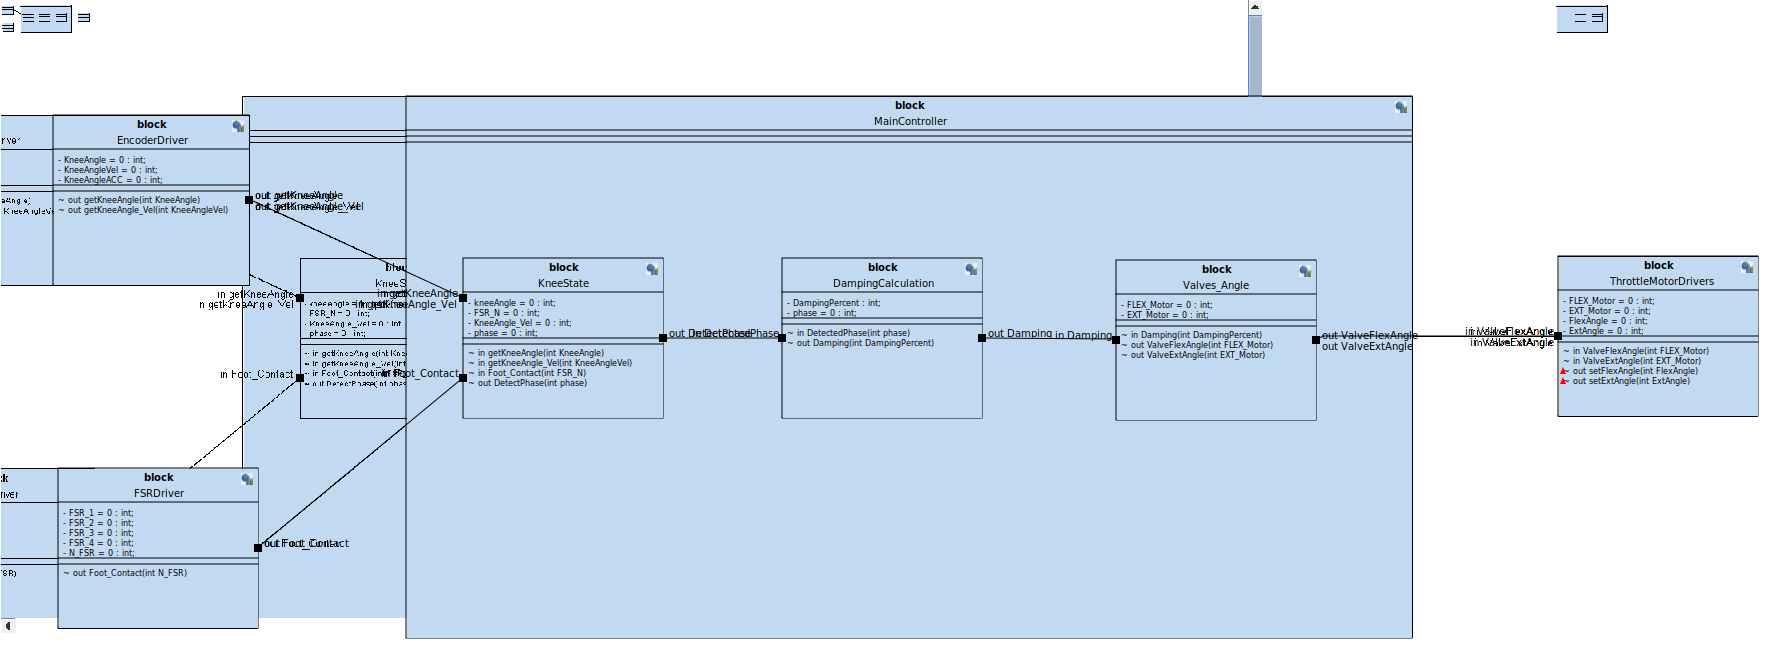
\includegraphics[width=\textwidth]{img_2_0.png}
\caption{Diagram "Block Diagram"}
\label{fig:Block DiagramBlock Diagram20}
\end{figure*}

\subsection{Behavior of Block: MainController}
Figures \ref{fig:MainControllerMainController21} presents ...
\begin{figure*}[htb]
\centering
\includegraphics[width=\textwidth]{img_2_1.png}
\caption{Diagram "Behavior of Block: MainController"}
\label{fig:MainControllerMainController21}
\end{figure*}

\subsection{Behavior of Block: FSR\_Driver}
Figures \ref{fig:FSRDriverFSRDriver22} presents ...
\begin{figure*}[htb]
\centering
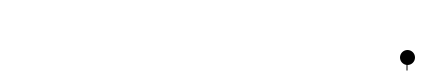
\includegraphics[width=\textwidth]{img_2_2.png}
\caption{Diagram "Behavior of Block: FSR\_Driver"}
\label{fig:FSRDriverFSRDriver22}
\end{figure*}

\subsection{Behavior of Block: ThrottleMotor\_Drivers}
Figures \ref{fig:ThrottleMotorDriversThrottleMotorDrivers23} presents ...
\begin{figure*}[htb]
\centering
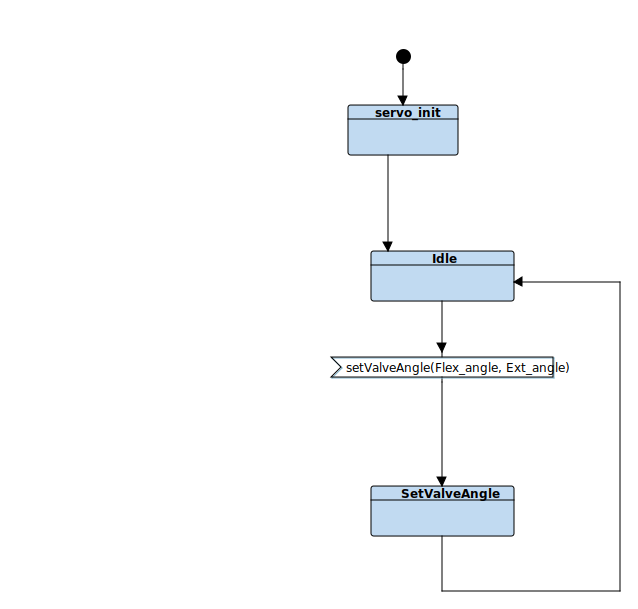
\includegraphics[width=\textwidth]{img_2_3.png}
\caption{Diagram "Behavior of Block: ThrottleMotor\_Drivers"}
\label{fig:ThrottleMotorDriversThrottleMotorDrivers23}
\end{figure*}

\subsection{Behavior of Block: Encoder\_Driver}
Figures \ref{fig:EncoderDriverEncoderDriver24} presents ...
\begin{figure*}[htb]
\centering
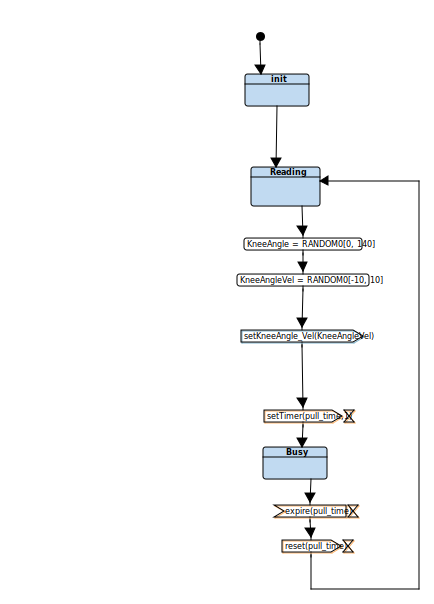
\includegraphics[width=\textwidth]{img_2_4.png}
\caption{Diagram "Behavior of Block: Encoder\_Driver"}
\label{fig:EncoderDriverEncoderDriver24}
\end{figure*}

\subsection{Behavior of Block: Gait\_Event}
Figures \ref{fig:GaitEventGaitEvent25} presents ...
\begin{figure*}[htb]
\centering
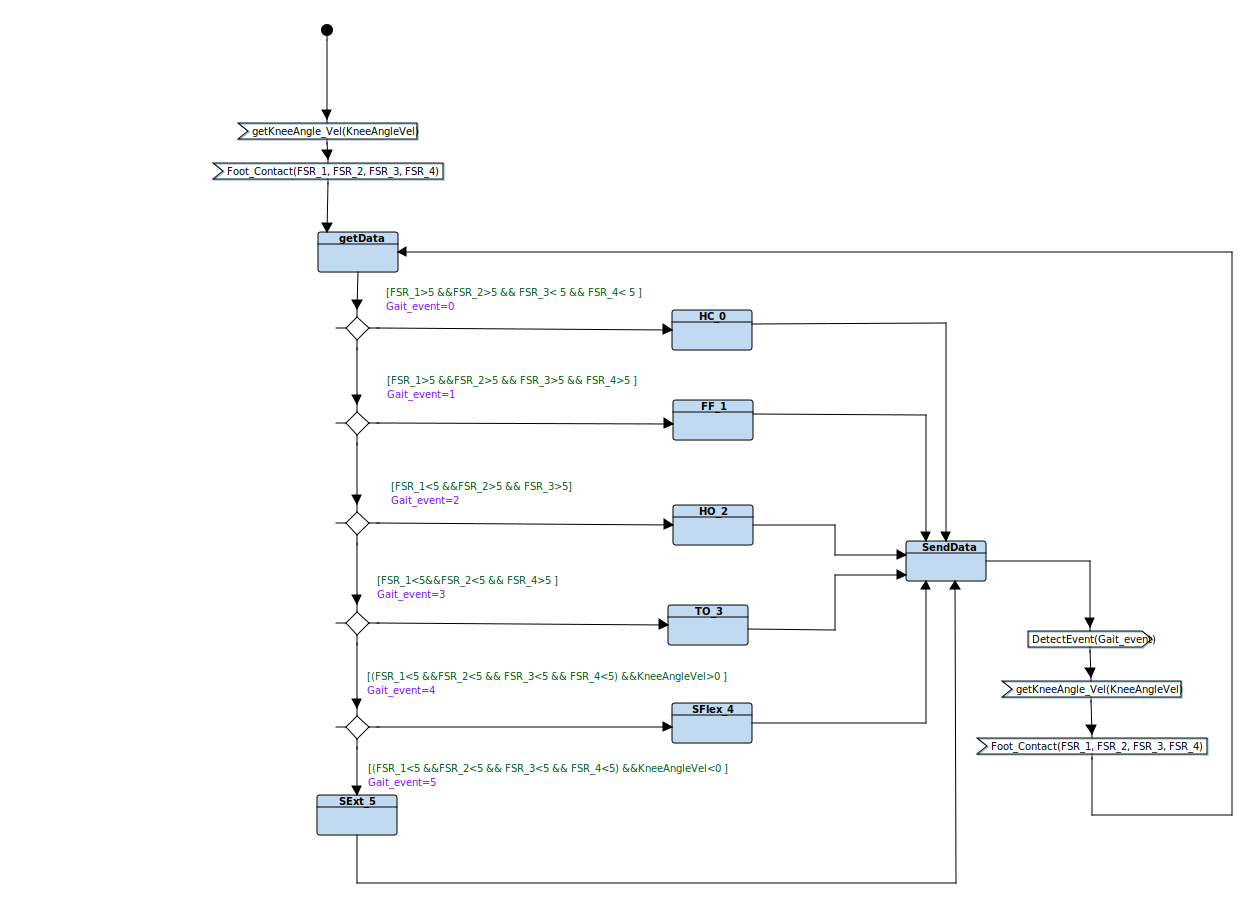
\includegraphics[width=\textwidth]{img_2_5.png}
\caption{Diagram "Behavior of Block: Gait\_Event"}
\label{fig:GaitEventGaitEvent25}
\end{figure*}

\subsection{Behavior of Block: Damping\_Control}
Figures \ref{fig:DampingControlDampingControl26} presents ...
\begin{figure*}[htb]
\centering
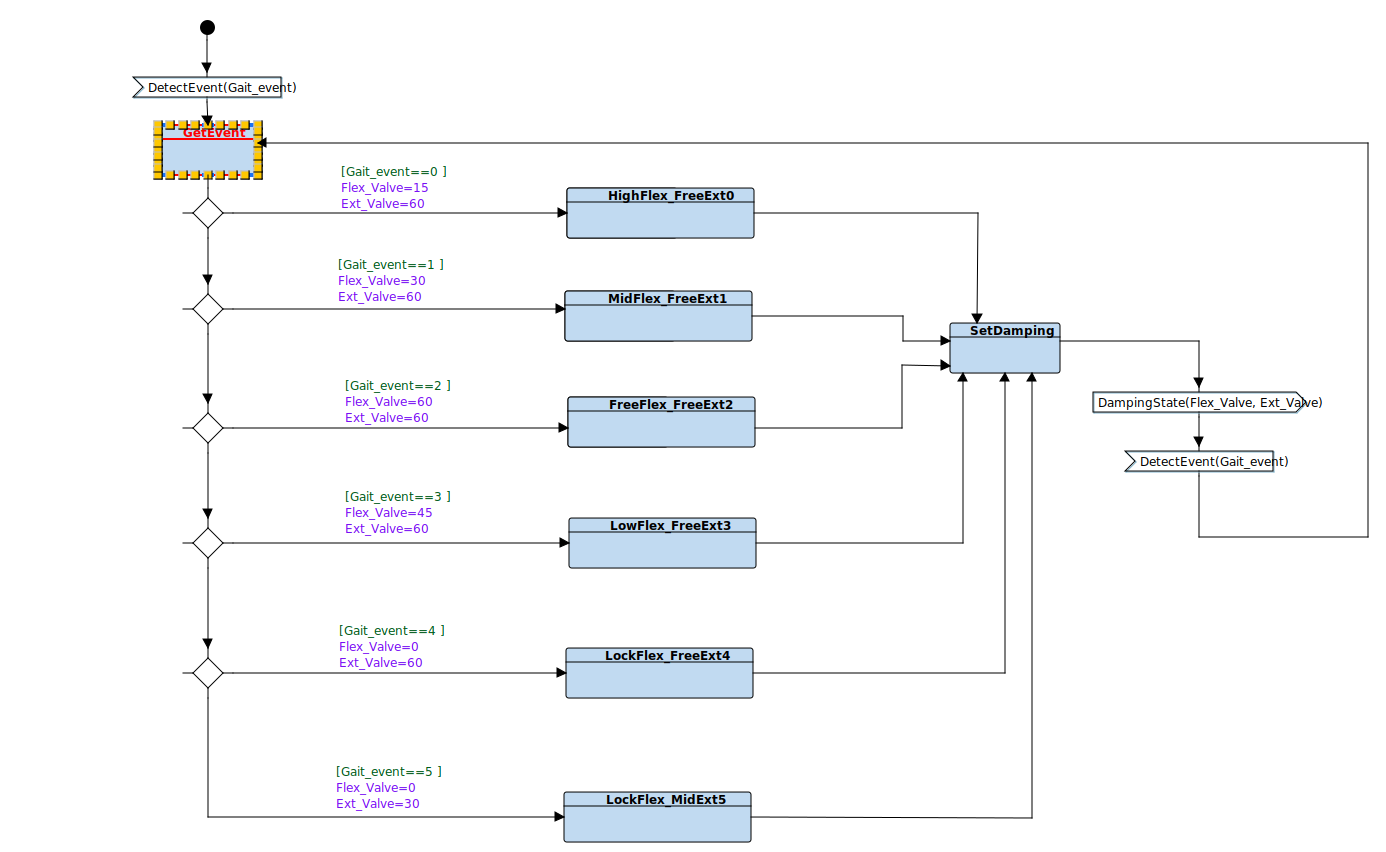
\includegraphics[width=\textwidth]{img_2_6.png}
\caption{Diagram "Behavior of Block: Damping\_Control"}
\label{fig:DampingControlDampingControl26}
\end{figure*}

